\chapter{Installation for Unix platform}\label{sec:InstallUnix}

\paragraph{}The FA$\mu$ST project is based on an C++ library available for both UNIX and Windows environments. CMake has been choose to build the project FA$\mu$ST because it is an open-source, cross-platform family of tools designed to build, test and package software.

\paragraph{}This chapter presents the steps to install the FA$\mu$ST tools on the Unix platform (both Linux and Mac OS). First section \ref{sec:UnixGettingStarted} presents the basic installation of FA$\mu$ST and second section \ref{sec:UnixCustomInstall} corresponds to the advanced  installation.

\section{Getting Started}\label{sec:UnixGettingStarted}

\subsection{Required tools}\label{sec:RequiredTools}

\begin{itemize}
\item CMake : (tested with version 3.4.3 cf. website \url{https://cmake.org/})
\item Matlab : (tested with version 2014 and 2015)
The use of the mex function in Matlab requires that you have a third-party compiler installed on your system. The latest version of Matlab (2016a in our case) only supports up to GCC 4.7 (see \url{http://fr.mathworks.com/support/compilers/R2016a/index.html?sec=glnxa64} for more detail). Please adjust your version of GCC compiler in order to run the installation properly. 
You must too have matlab in your environment PATH. If not please add. 

\item \textit{OPTIONAL} The use of GPU process in FAUST project required the drivers for NVIDIA and CUDA install. You must have nvcc in your environment PATH. If not please add.
\end{itemize}

\paragraph{}Please export following variable:
\begin{itemize}
\item CC with gcc (example: "\texttt{export CC='/usr/lib64/ccache/gcc'}") 
\item CXX with g++ (example: "\texttt{export CXX=/usr/lib64/ccache/g++}
\end{itemize}

\subsection{Required packages}\label{sec:RequiredPackages}

\paragraph{}Here is a list of packages used in the FA$\mu$ST project. Normally, the installation of this packages are automatically done (see the directory "./externals").
\begin{itemize}
\item eigen
\item openBlas
\item xml2
\item matio
\end{itemize}

\subsection{Basic build and installation}\label{sec:UnixBuildInstall}
\paragraph{}When prerequisities listed in precedent sections are checked, the FA$\mu$ST installation can be done : 

\begin{itemize}
\item Download the FA$\mu$ST package on the website :  \url{http://faust.gforge.inria.fr/}
\item Open a command terminal
\item Place you in the FA$\mu$ST directory, and type the following commands : 
\begin{lstlisting}
mkdir build
cd build
cmake ..
make
make install
\end{lstlisting}
\end{itemize}

\paragraph{}When using the \texttt{cmake} command to generate the build system, Cmake performs a list of tests to determine the system configuration and manage the build system. If the configuration is correct then the build system is generated and written. In this case the three last lines of the console log of cmake command should be: \\
\texttt{... \\
-- Configuring done \\
-- Generating done \\
-- Build files have been written to: ./build}

\paragraph{}The command \texttt{make} will compile the build files.

\paragraph{}The command \texttt{make install} will install in default directory.



\section{Custom - Advanced Installation}\label{sec:UnixCustomInstall}

\paragraph{}The project FA$\mu$ST can be configured with optional parameters, for example if you want to install FA$\mu$ST in a different folder or to enable the parallel computing using multithread capacities provided by the OS. This build system can be parametrized using the Cmake Graphical User Interface, or the Cmake command line tools. 

\paragraph{}The Cmake Graphical User Interface ccmake allows you to selected option input. When using the \texttt{ccmake} command in your build directory, the Cmake GUI appears in the console (see figure \ref{fig:ccmake}).

\begin{figure}[!htbp]
\label{fig:ccmake}
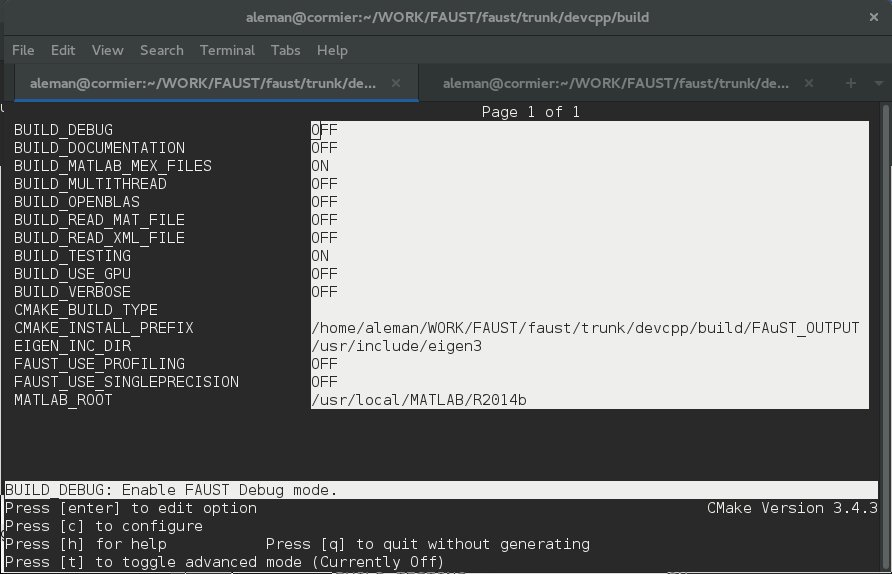
\includegraphics[scale=0.5]{images/ccmake.jpg}
\end{figure}

\paragraph{}When scrolling on a value and pressing [enter], this value can be edited, the black underlaid row displays some information about the option and required path to create the build system. In the case of an option press [enter] to toggle the ON/OFF values.
\paragraph{}After choosing options for the build and setting the required fields, press [c] to configure. The configuration of the build system is checked again by Cmake, at the end of this check if the build settings are correct, you can press [g] in order to generate the build system.
	

\paragraph{} Instead the ccmake GUI, an other possibility to configure and generate the project is to use the command line cmake which can take the option input. Here is the list of available options: 
\texttt{$cmake\ ..\ -D<BUILD\_NAME>=<ON/OFF>$}

\begin{itemize}
\item BUILD\_TESTING : Enable the ctest option (default value is ON)
\item BUILD\_DOCUMENTATION : Generating the doxygen documentation (default value is OFF)  
\item BUILD\_MULTITHREAD : Enable multithread with OpenMP Multithreading (default value is OFF)
\item BUILD\_VERBOSE : Enable verbose option when compile (-v) (default value is OFF)
\item BUILD\_DEBUG : Enable FAUST Debug mode (default value is OFF )
\item BUILD\_USE\_GPU : Using both CPU and GPU process ( default value is OFF)
\item BUILD\_MATLAB\_MEX\_FILES : Enable building Matlab MEX files (default value is ON)
\item BUILD\_OPENBLAS : Using openBLAS for matrix and vector computations (default value is OFF )
\item BUILD\_READ\_XML\_FILE : Using xml2 library to read xml files (default value is OFF)
\item BUILD\_READ\_MAT\_FILE : Using matio library to read mat files (default value is OFF)
\end{itemize}

\paragraph{}Following the selected option, the cmake installer automatically checks the dependent component (library OpenBlas, eigen, matio, libxml2).  

\section{Build using Code Block}\label{sec:UnixInstallCodeBlock}
progress...
